% Chapter Template


\chapter{Evidence of active aggregation behaviour in \emph{Lucilia sericata} larvae and possible implication of a conspecific mark} % Main chapter title

\label{Chapter2} % Change X to a consecutive number; for referencing this chapter elsewhere, use \ref{ChapterX}

\lhead{Chapitre 2. \emph{Evidence of active aggregation behaviour of larvae and possible implication of a conspecific mark}} % Change X to a consecutive number; this is for the header on each page - perhaps a shortened title

Julien \textsc{Boulay}\up{a,b}, Cédric \textsc{Devigne}\up{a,c}, Didier \textsc{Gosset}\up{a} and Damien \textsc{Charabidzé}\up{a}

\up{a} Univ. Lille, CHU Lille, EA 7367 - UTML - Unité de Taphonomie Médico-Légale, Lille, France\\
\up{b} Université Libre de Bruxelles, Unit of Social Ecology, Brussels, Belgium\\
\up{c} UCLille, FLST, Laboratoire Ecologie et Biodiversité, Lille, France\\


Article publié dans \emph{Animal Behaviour}, 85:6, 1191-1197, 2013.

\cleardoublepage

%----------------------------------------------------------------------------------------
%	SECTION 1
%----------------------------------------------------------------------------------------
\section{Highlights}
\begin{itemize} 
\item[\tiny{$\blacksquare$}] The aggregation took place quickly and increased with time.
\item[\tiny{$\blacksquare$}] Our results suggest that thigmotaxis affects larval distribution.
\item[\tiny{$\blacksquare$}] Our results suggest that larvae deposit a mark that is detected by the other larvae.
\item[\tiny{$\blacksquare$}] Larvae are able to detect and to stay in the zone where this signal is deposited.
\item[\tiny{$\blacksquare$}] This mark is a potential vector of aggregation in this species.
\end{itemize}


%----------------------------------------------------------------------------------------
%	SECTION 2
%----------------------------------------------------------------------------------------

\section{Abstract}

Vectors of aggregation are well known for some arthropod species, but not for many others. We aimed to describe larval aggregation (experiment 1) in the carrion fly, \textit{Lucilia sericata} (Diptera: Calliphoridae), and to investigate the effect of food and conspecifics on larval behaviour (experiment 2). In experiment 1, 40 larvae were placed in a petri dish with a homogeneous diet for 30min, 1h, 3h, 5h or 24h. This experiment demonstrated for the first time under controlled conditions the active aggregation of \emph{L. sericata} larvae. The results indicate that the aggregation took place quickly and was reinforced with time. After only 3h, one main aggregate comprising a majority of individuals was observed. These results also highlight the likely use by necrophagous larvae of a signal left by conspecifics as an aggregation vector. In experiment 2, we used a video-tracking system to investigate whether such an aggregative signal exists. Fed and starved larvae were tracked for 5 min in a circular area with each half marked with a different signal combination. The time spent in the signal zones, the distance travelled, the velocity, the time at the stop and the number of stops in each zone were measured. The larvae were significantly retained by a signal (mark) left by conspecifics. Together, the results of this study demonstrate the existence of a contact and/or odour-mediated signal involved in the aggregative behaviour of necrophagous larvae.

\emph{Keywords:} binary choice - blow fly larva - gregariousness - individual distribution - larval mass - \textit{Lucilia sericata} - retentive signal - self-organization - thigmotaxis - video tracking.

\clearpage
%----------------------------------------------------------------------------------------
%	SECTION 3
%----------------------------------------------------------------------------------------

\section{Introduction}

Blow flies (Diptera: Calliphoridae) are mostly oviparous. Females lay their eggs on carcasses, and the hatched larvae feed on the decaying meat. Blow flies are usually found in large masses of hundreds to thousands of larvae \citep{ives_aggregation_1991,slone_thermoregulation_2007}. One of the most impressive consequences of these aggregations of necrophagous dipteran larvae is the elevation of temperature inside the aggregation \citep{slone_thermoregulation_2007, charabidze_larval-mass_2011}. This local increase in temperature can reach 25\up{o}C above ambient temperature and is strongly correlated with the number of larvae \citep{charabidze_larval-mass_2011}. Furthermore, temperature inside larval masses appears to be regulated by several feedback loops, such as the evaporation of humidity from the individuals towards the surface, which could accentuate the cooling phenomenon \citep{slone_thermoregulation_2007, nelson_thermal_2009, rivers_physiological_2011}. Because the development of blow fly larvae is temperature dependent \citep{huckesfeld_feel_2011}, their gregarious behaviour may be an efficient mechanism to reduce development time and thus increase larval survival. Furthermore, aggregation prevents larval desiccation, decreases the risk of predation \citep{putman_dynamics_1977} and allows insects to exploit resources better \citep{hobson_studies_1932}. Thus, aggregation behaviour appears to be fundamental for the survival of necrophagous larvae \citep{slone_thermoregulation_2007, nelson_thermal_2009}. Gregariousness in necrophagous larvae is consistent with the Allee effect theory \citep{stephens_consequences_1999}, which asserts that the presence of many congeners in a single place confers benefits on all individuals \citep{stephens_consequences_1999, etienne_interaction_2002, woodcock_aggregation_2002, allen_group_2010}.

In such cases, self-organization theory is often invoked to explain how complex collective behaviour, such as aggregation, can emerge from simple individual interactions \citep{deneubourg_collective_1989,bonabeau_self-organization_1997,bonabeau_auto-organisation_1997,camazine_self-organization_2001,sumpter_collective_2009}. In this context, the aggregation behaviour exhibits positive feedback on insect behaviour at the individual level \citep{bonabeau_auto-organisation_1997}. This positive feedback allows an amplification of the system and generates a particular structure (e.g. the aggregation). This feedback is possible only if communication exists between group members \citep{deneubourg_dynamics_2002}.

The aggregation signals used by necrophagous dipteran larvae have been little studied and are poorly understood. To our knowledge, no experimental study has yet considered the signal underlying the aggregation behaviour of necrophagous calliphorid larvae. Because larvae are aggregated upon hatching (females lay clusters of hundreds of eggs on carcasses, which possibly plays a role in the aggregation), one can ask whether a signal is used to initiate and/or stabilize the aggregation. In this context, we focused on testing two points: (1) whether carrion fly, \textit{Lucilia sericata}, larvae have an efficient gregarious behaviour under controlled conditions and (2) whether the previous presence of larvae is a retentive signal for subsequent conspecifics.


%----------------------------------------------------------------------------------------
%	SECTION 4
%----------------------------------------------------------------------------------------
\section{Material and Methods}

%-----------------------------------
%	SUBSECTION 1
%-----------------------------------

\subsection{Insect rearing}
The experiments were performed on \textit{L. sericata} larvae that were obtained from rearing colonies bred at the Forensic Institute of Lille (Nord, France). Adults were reared at ambient temperatures (25 $\pm$2\up{o}C) and natural light. Flies were fed ad libitum with caster sugar and water. Beginning with the adult fly emergence (day 0), minced beef liver was added for 7 days (day 7) to provide the proteins necessary for vitellogenesis. After 5 days with no food, liver was again provided to trigger egg laying (day 12). Eggs were placed on the breeding substrate (100g of fresh minced liver), and the temperature was set to 17 $\pm$0.5\up{o}C (day 13). Only those larvae aged between 5 and 6 days (day 18–19, corresponding to young third instars, 10 $\pm$2mm long) were used for experiments \citep{grassberger_effect_2001}. At this age, larvae have the same sensory responses as second-instar larvae \citep{cobb_what_1999}.

%-----------------------------------
%	SUBSECTION 2
%-----------------------------------

\subsection{Experiment 1: Larval Aggregation Over Time}
Forty larvae were randomly introduced into a glass petri dish (diameter = 17cm) filled to 1cm depth with a homogeneous diet. The diet was made of 20g of agar, 50g of yeast and 20$\%$ pig's blood diluted in 1 litre of water \citep{daniels_simple_1991}. The temperature of the dishes was maintained at 25\up{o}C during time t (0h, 0.5h, 1h, 3h, 5h and 24h). After time t, the dishes were instantaneously divided into 4cm\up{2} squares using a plastic lattice, creating a total of 54 quadrats. The number of larvae present in each quadrat was counted. An aggregation was defined as a peak number of individuals in a single quadrat. Because we had to destroy their environment to count the larvae that were present in each quadrat, we performed only five replicates for each observation time.

The distribution index I was calculated for each replicate r to estimate the intensity of aggregation. The index is given by Ir = $\frac{SD\up{2}}{\mu}$ where $\mu$ is the mean percentage of individuals observed among all quadrats, and SD is the standard deviation \cite{canard_quelques_2004}. In some replicates, a few larvae were lost during the counting. To homogenize the data, we used the mean percentage of individuals in the calculation of I instead of the mean number.

The radial distribution of the individuals was obtained by dividing the arena into three concentric circles with radii of r$_{1}$ = 3cm, r$_{2}$ = 6cm and r$_{3}$ = 8.5cm. The percentage of individuals present in each circle was noted and compared to a theoretical distribution. This method is described in detail in \citet{sempo_integration_2006}.

%-----------------------------------
%	SUBSECTION 3
%-----------------------------------

\subsection{Experiment 2: Effects of Signals on Behaviour}
Prior to the experiments, the larvae were removed from the breeding substrate, placed in wet pine sawdust and isolated in the dark at 25 $\pm$1\up{o}C. This isolation time starved the larvae and decreased their stress, while the sawdust removed traces of food from their cuticle. Two groups of larvae were tested: (1) larvae that had been isolated from the breeding substrate for 30min (fed larvae) and (2) larvae that had been isolated for 240min (starved larvae without food in their crop; according to data we collected by dissecting 10 crops, this amount of time is sufficient to starve the larvae; the mean surface area of crops was 3.4 $\pm$1.8mm\up{2} for fed larvae and 0.5 $\pm$0.2mm\up{2} for starved larvae; Mann–Whitney U test: U = 117.5, P $<$ 0.001). Larvae of the two tested groups (i.e. fed and starved larvae) were individually tracked for 5min in a binary choice test. Preliminary tests indicated that 5min was sufficient time for larvae to make a choice.

The experimental set-up consisted of a 2 cm tall cellulose Petri dish (diameter = 9cm) with a glass cover. This arena was lit from below by a dark light tube at a distance of 15cm (15W; $\lambda$ = 320–380nm). The wavelength was not perceivable by larvae \citep{strange_spectral_1961} and thus prevented any stress from light \citep{hinnemann_see_2010}. During the experiments, the temperature of the set-up was maintained at 25 $\pm$1\up{o}C in a thermostatic chamber. Because circadian activity does not affect larval locomotion behaviour \citep{joplin_effects_1999}, experiments were performed daily from 0900 to 1800 hours. After each trial, the arena and the glass cover were cleaned in a methanol bath for 2min at 20\up{o}C in an ultrasonic cleaner (Bioblock Scientific 86484) and washed with water.

The arena was virtually divided in half (equal zones) using the video-tracking software Ethovision 8.5XT (Noldus Information Technology, Wageningen, The Netherlands). The two zones corresponded to areas in which test signals were deposited. For each trial, a clean, wet, absorbent sheet of paper lined the bottom of the dish. The signals were deposited directly onto the absorbent paper. Larvae were then placed at the centre of the arena and followed by the video-tracking system. A digital camera (Bosch Dinion LTC0355; resolution: 752 $\times$ 582) was used to record larval displacement. The data were analysed using the video-tracking system. The time spent in the signal zones, distance travelled, velocity, time of each stop and number of stops in each zone were measured.

One control and two signals, Food and Larvae, were tested. In the Control trials, no test signals were deposited. The Food trials consisted of 100$\mu$l of a solution containing 3g of beef liver diluted in 50ml of distilled water. The test signal was deposited such that the signal spread over the entire zone (half of the arena). The Larvae trials included the marks created by five ‘signal’ larvae. Prior to depositing the test signals, signal larvae were starved and cleaned for 1h in wet sawdust to eliminate any food odours acquired in the breeding substrate. The signal larvae were then confined to one half of the petri dish and were free to crawl for 10 min. These larvae were removed before the start of the trials. Observations of the movement of the signal larvae indicated that their markings were homogeneously distributed on the entire half of the petri dish surface to which they were confined. One control and three binary choice combinations of these signals were tested: Control, Control versus Larvae (C versus L), Control versus Food (C versus F) and Larvae versus Food (L versus F).

%-----------------------------------
%	SUBSECTION 4
%-----------------------------------

\subsection{Statistical Analysis}
The Z test was used to test individual distribution during experiment 1. The random distribution hypothesis can be rejected if the absolute value of Z is greater than 1.96 \cite{canard_quelques_2004}. If the index of distribution I is less than 2.5, the distribution is regarded as homogeneous. If I $>$ 2.5, the distribution is considered aggregative.

The data were not normally distributed (Kolgomorov–Smirnov test), and the assumption of variance homogeneity was true (Bartlett's test). Following \citet{zar_biostatistical_2010}, the Wilcoxon signed-ranks test was used to compare the amount of time spent in either zone during each experimental trial. The total distance travelled, distance travelled in each zone, velocity in each zone, time of each stop and number of stops were analysed using nonparametric tests (Kruskal–Wallis, Wilcoxon and Mann–Whitney). Tests were performed using XLSTAT version 2011.1.03 (Addinsoft, New York, U.S.A.) and GraphPad InStat version 3.06 for Windows. All analyses used a significance level of $\alpha$ = 0.05, unless otherwise stated. For the Dunn's multiple paired comparison tests, the significance level $\alpha$ was adjusted using the Bonferroni method.


%----------------------------------------------------------------------------------------
%	SECTION 5
%----------------------------------------------------------------------------------------

\section{Results}

%-----------------------------------
%	SUBSECTION 1
%-----------------------------------

\subsection{Experiment 1: Larval Aggregation Over Time}
At the start of each trial, larvae were randomly distributed in the petri dish; the index mean at t = 0 was not significantly different from I$_{random}$ (I$_{random}$ = 2.5; I$_{t=0}$ = 3 $\pm$0.5, NS). All values of I were significantly higher than that for random distribution (I$_{random}$ = 2.5; Figure \ref{fig:agreg}), which indicated that individuals were aggregated. Aggregation was observed after 0.5h (I$_{t=0.5h}$ = 11.9 $\pm$2.1, Z = 25.3, P $<$ 0.001); however, the number of isolated individuals at t = 0.5h remained high (80$\%$ of the larvae; Figure \ref{fig:agreg}). Aggregations were mainly located at the periphery of the Petri dish, in contact with the wall (Figure \ref{fig:agreg}). The number of larvae in the largest aggregation increased with time. After 3h, more than 60$\%$ of the larvae were gathered in a single aggregation (I$_{t=1h}$ = 14.1 $\pm$7.7, Z = 28.5, P $<$ 0.001; I$_{t=3h}$ = 35.2 $\pm$23.2, Z = 50.9, P $<$ 0.001; Figure \ref{fig:agreg}). After 5h, a main aggregation containing more than 70$\%$ of the larvae was observed in each trial (I$_{t=5h}$ = 45.5 $\pm$18.4, Z = 59.2, P $<$ 0.001; \ref{fig:agreg}). After 24h, only a few minor aggregations remained, and they were mainly located in the quadrats neighbouring the main aggregation (I$_{t=24h}$ = 46.3 $\pm$24.9, Z = 59.9, P $<$ 0.001; Figure \ref{fig:agreg}). The mean index increased with time, which indicated that larvae were increasingly aggregated (Kruskal–Wallis test: T = 14.6, P $<$ 0.01; Dunn's test: I$_{t=0.5h}$ $\neq$ I$_{t=5h}$, I$_{t=0.5h}$ $\neq$ I$_{t=24h}$, I$_{t=1h}$ $\neq$ I$_{t=5h}$, I$_{t=1h}$ $\neq$ I$_{t=24h}$, P $<$ 0.01). The results of the radial distribution experiment indicated that the majority of the individuals at each observation time were located near the arena's edge, except after 24 h (Figure \ref{fig:rad}).

\begin{figure}[h]
	\centering
		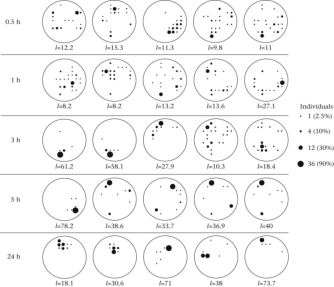
\includegraphics[width=0.9 \textwidth]{Figures/agreg_animbehav.pdf}
		\rule{35em}{0.5pt}
	\caption[Agregation]{Number of larvae aggregated in relation to time. Each large circle corresponds to one independent experiment. The sizes of black circles are proportional to the number of larvae present (40 larvae were used in each replicate). I: index of distribution corresponding to (SD)\up{2}/mean. The I for a random distribution is 2.5 and the I$_{mean}$ at t = 0 is 3 $\pm$0.5.}
	\label{fig:agreg}

\end{figure}

\clearpage

\begin{figure}[t]
\centering
		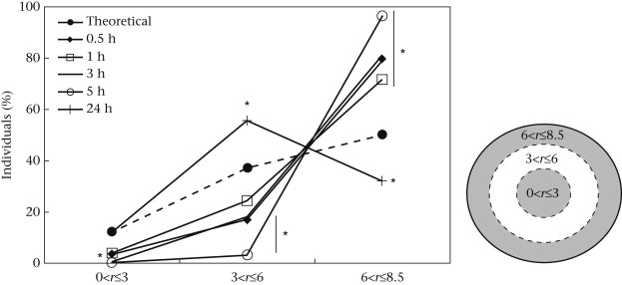
\includegraphics[width=0.8 \textwidth]{Figures/rad_animbehav.png}
		\rule{35em}{0.5pt}
		\caption[Radial]{Spatial localization of the larvae in the arena (virtually divided into three concentric circles) in relation to time (0.5, 1, 3, 5 and 24h). The theoretical distribution corresponds to a homogeneous distribution of individuals in the three concentric circles. Asterisks indicate significant differences from the theoretical distribution \\(chi-square test: N = 40 individuals).}
	\label{fig:rad}
    

\end{figure}



%-----------------------------------
%	SUBSECTION 2
%-----------------------------------

\subsection{Experiment 2: Effect of Signals on Behaviour}

\textit{Control trials}

In the Control trials, fed and starved larvae spent the same amount of time in both halves of the arena, indicating an unbiased experimental set-up (Table \ref{tab:table}, Figure \ref{fig:duree}). The distances travelled by fed and starved larvae and their velocities in each zone did not differ (Figures \ref{fig:distance} and \ref{fig:velocity}).

\textit{Control versus Signal trials}

Regardless of whether they were fed or starved, the larvae spent significantly more time in the Signal zone than in the Control zone (Table \ref{tab:table}, Figure \ref{fig:duree}). Both fed and starved larvae also traveled significantly greater distances in the Signal zone than in the Control zone (Figure \ref{fig:distance}) but moved at the same speed in each zone (Figure \ref{fig:velocity}).

In the Control versus Food trials, fed and starved larvae spent more time stationary and stopped more frequently in the Food zone than in the Control zone (Figures \ref{fig:downtime} and \ref{fig:stops}). In contrast, in the Control versus Larvae trials, fed larvae spent the same amount of time stationary and stopped the same number of times in the two zones (Figures \ref{fig:downtime} and \ref{fig:stops}). Starved larvae spent the same amount of time stationary in the two zones (Figure \ref{fig:downtime}), but they stopped more frequently in the Larvae zone than in the Control zone (Figure \ref{fig:stops}).

\clearpage


\textit{Signal versus Signal trials}

In the Larvae versus Food trials, larvae spent significantly more time in the Food zone. This result was observed regardless of whether the larvae were fed or starved (Table \ref{tab:table}, Figure \ref{fig:duree}). However, fed larvae travelled greater distances in the Food zone, whereas starved larvae travelled the same total distance in each zone (Figure \ref{fig:distance}). Unpaired comparisons of mean velocity in each zone between fed and starved larvae revealed that fed larvae moved more quickly than starved larvae in the Food zone (Figure \ref{fig:velocity}). In contrast, starved larvae spent more time and stopped more frequently in the Food zone (Figures \ref{fig:downtime} and \ref{fig:stops}).


\begin{table}[p]
	\centering
    \caption[Table]{Mean times $\pm$SD (s) spent by the fed and starved larvae in the two zones of the arena for each combination of signals}
    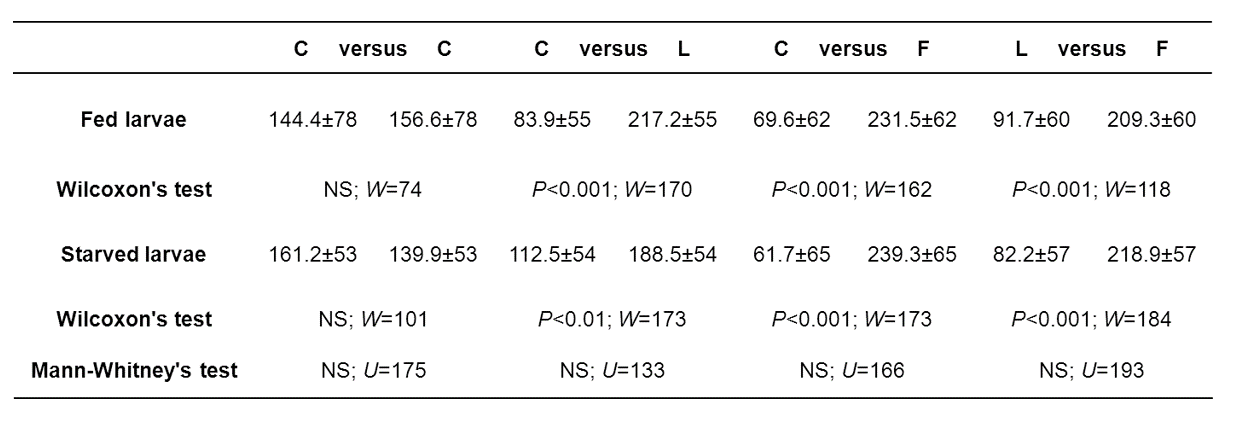
\includegraphics[width=0.9\textwidth]{Figures/table.png}
    \label{tab:table}
\end{table}

\begin{figure}[p]
	\centering
    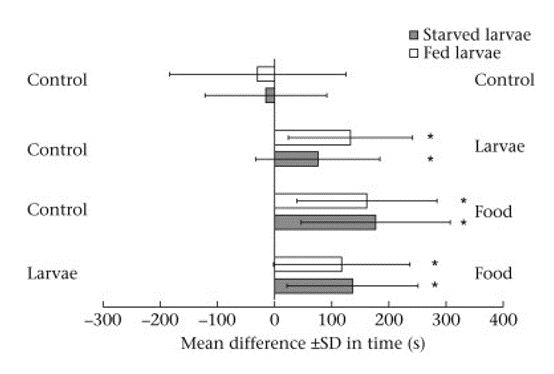
\includegraphics[width=0.9 \textwidth]{Figures/duree.png}
    \rule{35em}{0.5pt}
    \caption{Mean difference $\pm$SD in time (s) spent between signals (half zones) for fed and starved \textit{L. sericata} larvae. The mean difference was obtained by subtracting the time spent by larvae in the signal zone on the right-hand side from the time spent in the signal zone on the left-hand side. If positive, more time was spent in the former and if negative, more time was spent in the latter. Asterisks indicate significant differences between zones (Wilcoxon test: N = 20). No differences between fed and starved larvae were observed whatever the experimental condition.}
    \label{fig:duree}   

\end{figure}

\begin{figure}[p]
	\centering
    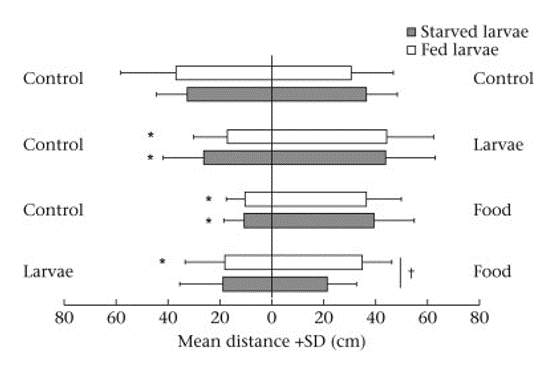
\includegraphics[width=0.8 \textwidth]{Figures/distance.png}
    \rule{35em}{0.5pt}
    \caption{Mean distances +SD (cm) travelled by fed and starved larvae in each zone of each experimental condition. Asterisks indicate significant difference between the mean distance travelled by larvae in the signal zone on the left-hand side and the mean distance travelled by larvae in the signal zone on the right-hand side (Wilcoxon test: N = 20). Dagger indicates significant difference between the mean distance travelled by fed larvae and the mean distance travelled by starved larvae in the same zone during the same condition (Mann–Whitney test: N = 20).}
    \label{fig:distance}  

	\centering
    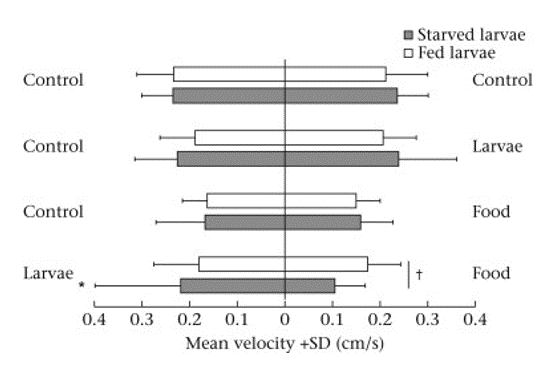
\includegraphics[width=0.8 \textwidth]{Figures/velocity.png}
    \rule{35em}{0.5pt}
    \caption{Mean velocities +SD (cm/s) recorded for fed and starved larvae in each zone of each experimental condition. Asterisks indicate significant difference between the mean velocity of larvae in the signal zone on the left-hand side and the mean velocity of larvae in the signal zone on the right-hand side (Wilcoxon test: N = 20). Dagger indicates significant difference between the mean velocity of fed larvae and the mean velocity of starved larvae in the same zone during the same condition \\(Mann–Whitney test: N = 20).}
    \label{fig:velocity}  
\end{figure}

\begin{figure}[p]
	\centering
    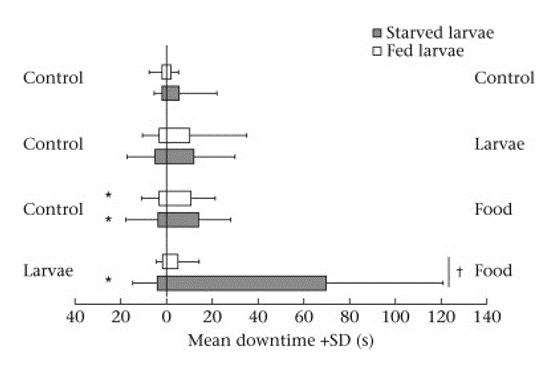
\includegraphics[width=0.85 \textwidth]{Figures/downtime.png}
    \rule{35em}{0.5pt}
    \caption{Mean time at the stop +SD (s) recorded for fed and starved larvae in each zone of each experimental condition. Asterisks indicate significant difference between the mean time at the stop of larvae in the signal zone on the left-hand side and the mean time at the stop of larvae in the signal zone on the right-hand side (Wilcoxon test: N = 20). Dagger indicates significant difference between the mean time at the stop of fed larvae and the mean time at the stop of starved larvae in the same zone during the same condition (Mann–Whitney test: N = 20).}
    \label{fig:downtime}  

	\centering
    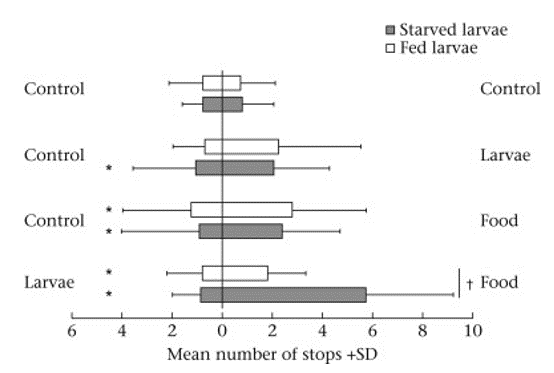
\includegraphics[width=0.85 \textwidth]{Figures/stops.png}
    \rule{35em}{0.5pt}
    \caption{Mean number of stops +SD recorded for fed and starved larvae in each zone of each experimental condition. Asterisks indicate significant difference between the mean number of stops of larvae in the signal zone on the left-hand side and the mean number of stops of larvae in the signal zone on the right-hand side (Wilcoxon test: N = 20). Dagger indicates significant difference between the mean number of stops of fed larvae and the mean number of stops of starved larvae in the same zone during the same condition (Mann–Whitney test: N = 20).}
    \label{fig:stops}  
\end{figure}

\clearpage

%----------------------------------------------------------------------------------------
%	SECTION 6
%----------------------------------------------------------------------------------------

\section{Discussion}
The gregariousness of necrophagous blow fly larvae has been extensively reported, especially in the context of forensic entomology, but rarely is the phenomenon studied under controlled conditions. In necrophagous species, aggregation behaviour is very well developed, and larvae aggregate in large masses of hundreds to thousands of congeners \citep{ives_aggregation_1991,slone_thermoregulation_2007}. This behaviour is assumed to have many benefits \citep{baxter_dynamics_1983, stephens_consequences_1999, slone_thermoregulation_2007, charabidze_larval-mass_2011, rivers_physiological_2011}, but the mechanisms of the process need to be clarified.

Our experiments showed that small aggregations appear over short timescales (0.5h) and gain more individuals over time. In other arthropod species, such as woodlice \citep{devigne_individual_2011,broly_aggregation_2012} and cockroaches \citep{jeanson_self-organized_2005}, the aggregations are formed more quickly, in approximately 5 min. Because cockroaches and woodlice move more quickly than \textit{L. sericata} larvae, the average velocity of these animals could explain the different timescales of their aggregations. The blow fly aggregations were located near the arena edge, except after 24h. These results illustrate the positive thigmotactic behaviour of blow fly larvae. Such observations have been reported in many arthropod species \citep{devigne_individual_2011, mailleux_collective_2011}. The large number of individuals present in the aggregation could explain the exception observed at 24h. After 24h, the aggregations included 30–40 larvae; the crawling effect, scramble competition and food consumption probably caused aggregations to move \citep{berrigan_how_1995}. Given this observation, the movement of the aggregation would be regulated by thigmotaxis for a small number of the larvae. In larger aggregations, the thigmotaxis between congeners is more important, as contact between congeners occurs more frequently than contact with the environment. To our knowledge, no studies have demonstrated whether such global movements are guided by a few individuals, as in human crowds \citep{dyer_consensus_2008}, primates \citep{sueur_selective_2009}  and the quorum effect \citep{sempo_complex_2009}. Furthermore, such displacement of an aggregation may simply result from mechanical phenomena (e.g. the crawling effect) and/or behavioural mechanisms (e.g. thermoregulation in the aggregation).

In mycophagous \textit{Drosophila} larvae, larval aggregation has been demonstrated to result from egg aggregation \citep{jaenike_aggregation_1991}. However, our results clearly showed that the aggregations of calliphorid larvae result from larval behaviour and are not solely attributable to the clustering of egg batches. Another common hypothesis regarding aggregation emphasizes the role of environmental heterogeneity \citep{mailleux_collective_2011, devigne_individual_2011, broly_aggregation_2012}. However, \textit{L. sericata} larvae that were randomly introduced into a homogeneous environment rapidly aggregated, and this aggregation increased with time. We conclude that the necrophagous fly larvae actively aggregate. This conclusion implies that the larvae used one or several mechanisms to gather, stabilize the aggregations and possibly move together \citep{zirbes_new_2010, mailleux_collective_2011}.

The video-tracking experiments clearly demonstrated, for the first time, the existence of a conspecific signal that can attract dipteran larvae to a given area. Our results suggest that \textit{L. sericata} larvae deposit a signal that is detected by other larvae. This signal had a movement-retentive effect and increased the amount of time that conspecifics remained in areas in which the signal was deposited. This result clearly showed not only that larvae can detect where conspecifics have been but also that they preferentially stay in those places. During the video-tracking experiments, we observed a mean velocity of 0.2 cm/s (Control trials), consistent with \citet{charabidze_modelisation_2010}. However, the presence of Food (signal) in the arena tended to decrease the mean velocity of starved larvae. Our observations indicated that starved larvae stopped and tried to eat the Food signal. This behaviour explains the decrease in the average velocity and the increase in the amount of time spent in the Food zone. The feeding behaviour is obviously related to the presence of food, but it also seems linked to the presence of other \textit{L. sericata} larvae. Indeed, in the Larvae versus Food trials, starved larvae spent more time stationary and stopped more frequently on the Food signal than the fed larvae in the Control versus Food trials. This behaviour suggests that the simultaneous presence of the two signals, although separate, influence the feeding behaviour of starved larvae. Larvae may be able to detect the larval signal from a distance, which would encourage them to feed \citep{devigne_out_2004}. Some previous studies have focused on the response of dipteran larvae to food signals \citep{christopherson_foraging_1997, cobb_what_1999, kaiser_behaviour_2008}, but no studies have addressed a possible interaction with signals deposited by conspecifics.

Lastly, both fed and starved larvae spent more time on the Food signal than on the Larvae signal (Larvae versus Food trials). Based on this result, we conclude that foraging behaviour prevails over aggregation behaviour in this species. However, the Larvae versus Food trial was a forced set-up; under natural conditions, larvae live on carcasses and thus never encounter such a choice. Furthermore, signals are deposited by larvae that have direct contact with the food source. To highlight the response of larvae to the signals deposited by congeners in an environment completely impregnated with food (seminatural conditions), experiments combining the signal larvae with the signal food are currently underway based on the same binary choice test set-up; however, these experiments combine the signal larvae with the signal food.

In addition, the young third-instar larvae used for these experiments may behave differently from one-instar or two-instar larvae. In contrast to third-instar larvae, young larvae have undeveloped mouth hooks. Because aggregation enhances the local liquefaction of tissues \citep{hobson_studies_1932}, younger larvae probably tend to aggregate to increase their access to soft food. This consideration is less important for older larvae, which can feed on solid tissues.

Our study addresses the question of aggregation mechanism at the collective level. Our experiments indicate that the aggregation of \textit{L. sericata} is an active, quick and efficient mechanism, probably mediated by larval signals. Thus, the gregarious behaviour of \textit{L. sericata} larvae probably results from dynamic processes that are mediated by attractive/retentive signals, and not only from thigmotaxis or environmental heterogeneity \citep{devigne_individual_2011, mailleux_collective_2011, broly_aggregation_2012}. Our observations at the scale of the individual also demonstrate that larvae deposit a signal that is perceived by conspecifics and has a movement-retentive effect. Together, these results strongly support the hypothesis that gregarious behaviour is mediated by a movement-retentive signal, which is deposited locally by conspecifics.

Further experiments should investigate the potential role of the larval signal on aggregation dynamics. Such data would facilitate models of larval mass over time in this and other insect species \citep{farine_gregarisme_1984, rivault_cockroach_1998, depickere_effect_2008}. Under natural conditions, larval aggregation can be interspecific \citep{amendt_current_2010} and it would be worth conducting studies of interspecific gregarious behaviour.

%----------------------------------------------------------------------------------------
%	SECTION 7
%----------------------------------------------------------------------------------------

\section{Acknowledgments}
J.B. and D.C. conceived and designed the experiments, J.B. performed the experiments, J.B. and D.C. analysed the data, J.B., D.C. and C.D. wrote the paper. Thanks to M. Daniau and E. Boulleaux for laboratory assistance and D. Toussaint for English correction. Thanks to J.-L. Deneubourg (Senior Research Associate from the F.R.S.-FNRS) for helpful suggestions and comments.


\clearpage




